\documentclass[fleqn,10pt]{wlscirep}
\title{Understanding Human Mobility Patterns from Semantic Twitter User Trajectories}

\author[1,*]{Junjun Yin}
\author[1]{xx}
%\author[1,2,+]{Christine Author}
%\author[2,+]{Derek Author}
\affil[1]{Department of Geography and Geographic Information Science}
\affil[ ]{University of Illinois at Urbana-Champaign, IL, 61801, USA}

\affil[*]{jyn@illinois.edu}

%\affil[+]{these authors contributed equally to this work}

%\keywords{Keyword1, Keyword2, Keyword3}

\begin{abstract}
xx
\end{abstract}
\begin{document}
\flushbottom
\maketitle
\thispagestyle{empty}

\section*{Introduction}
The Introduction section, of referenced text\cite{Figueredo:2009dg} expands on the background of the work (some overlap with the Abstract is acceptable). The introduction should not include subheadings.

The discovery and identifications of Lévy flight distribution, however, the implication of Lévy flight is that the process illustrates randomness.  


\section*{Results}

\begin{figure}[ht]


\centering
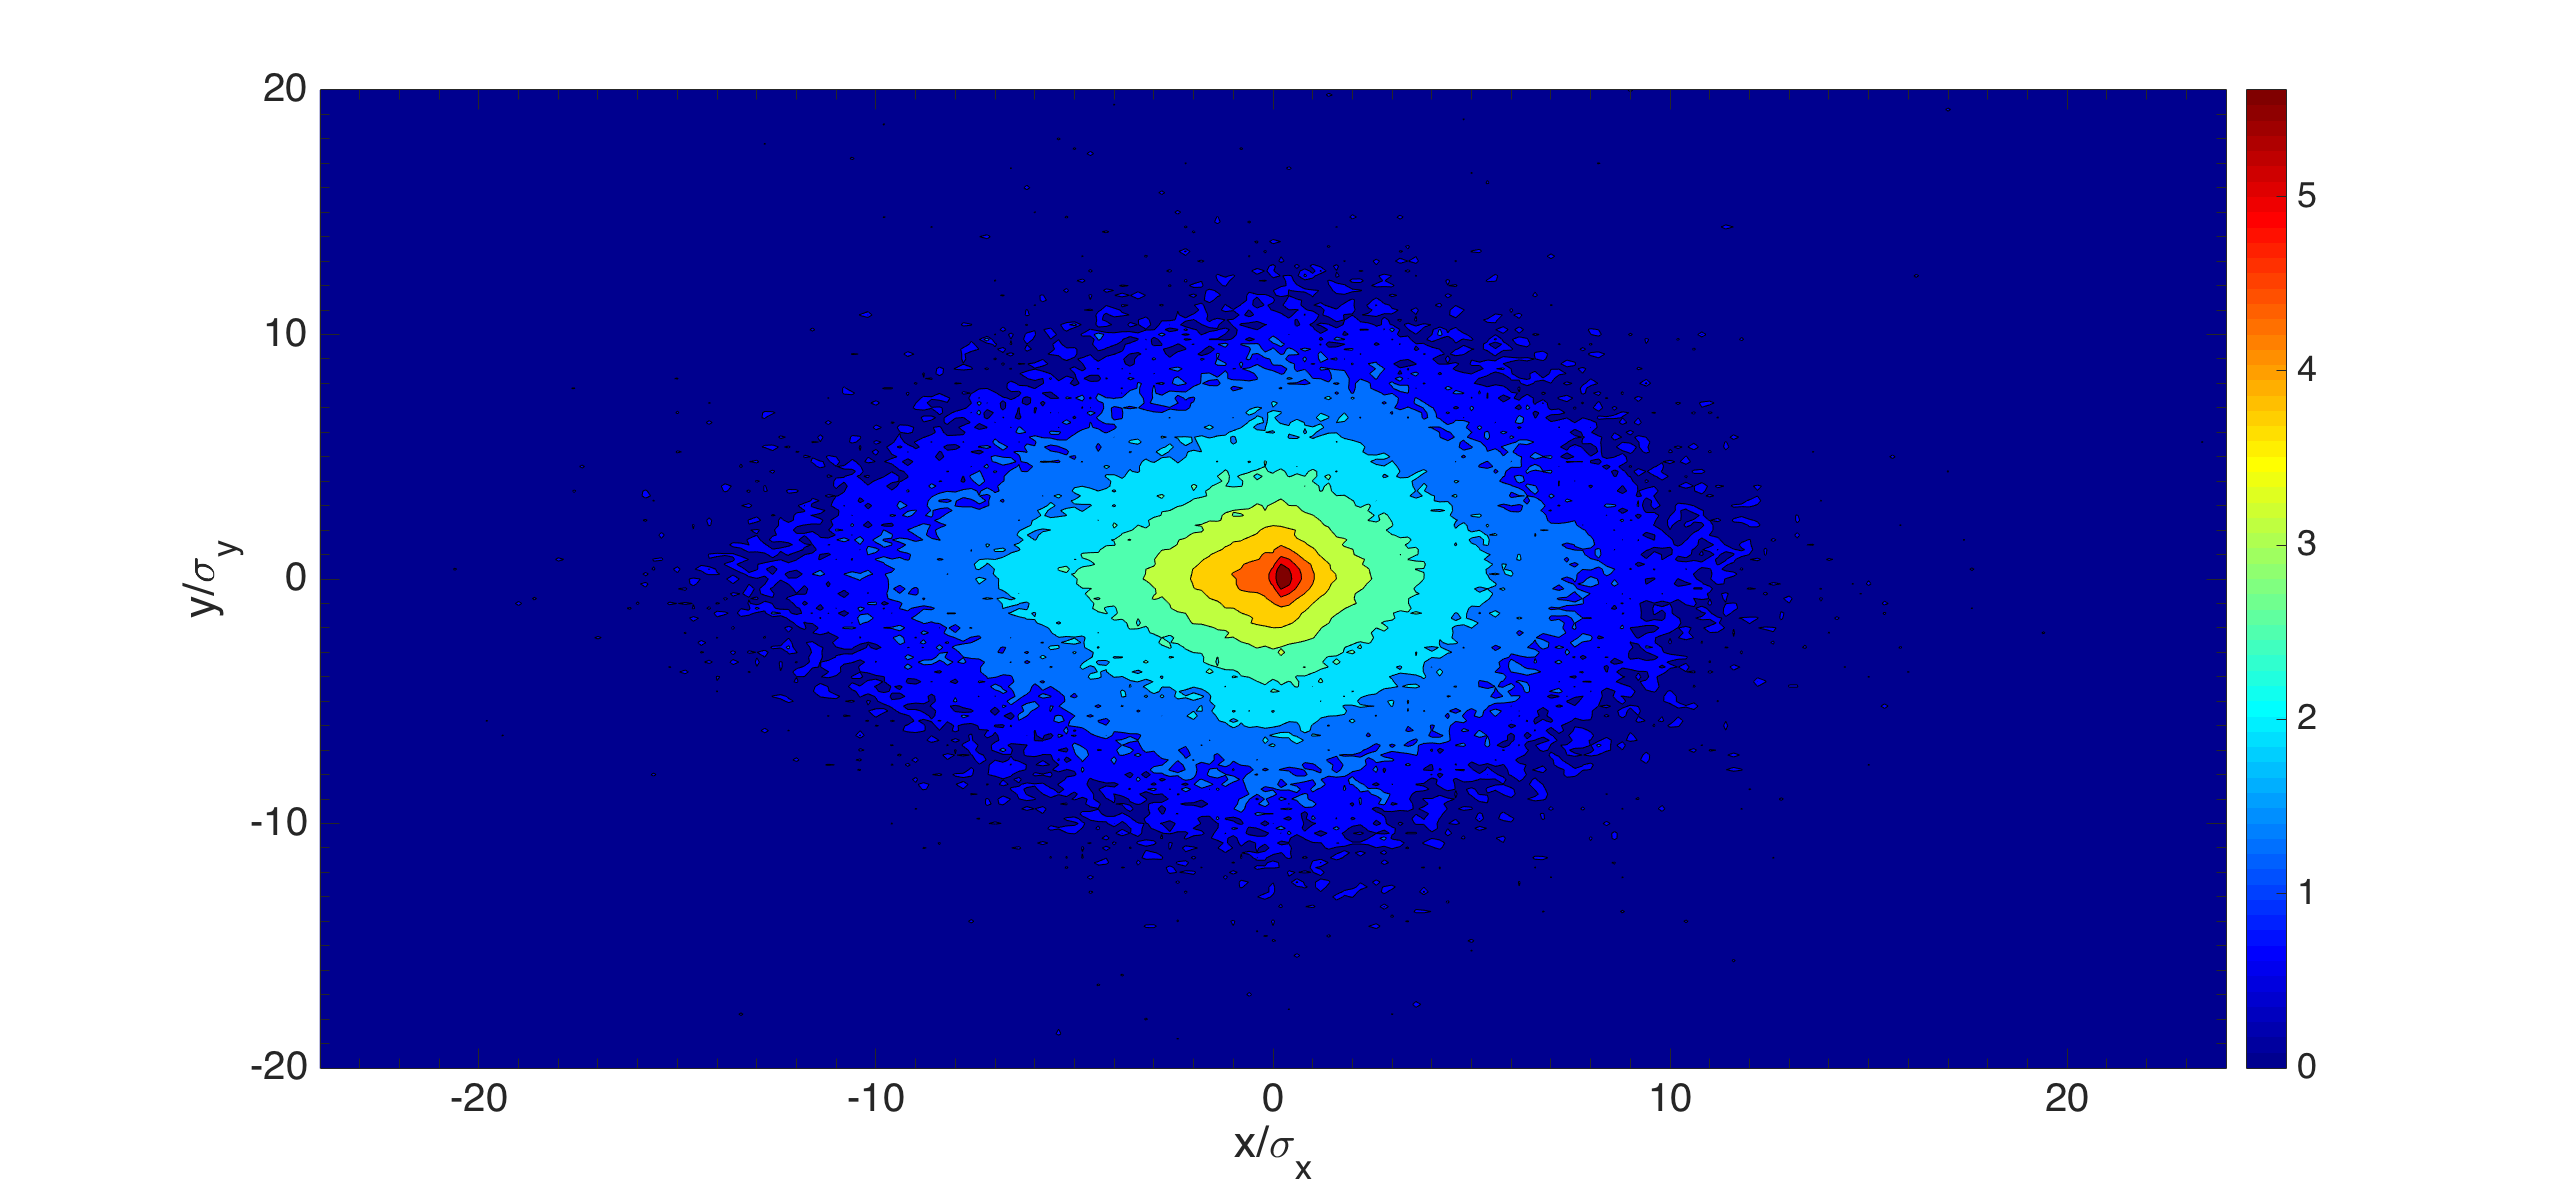
\includegraphics[width=\linewidth]{Chicago_Shape}
\caption{Legend (350 words max). Example legend text.}
\label{fig:Chicago_Shape}
\end{figure}


\begin{figure}[ht]
\centering
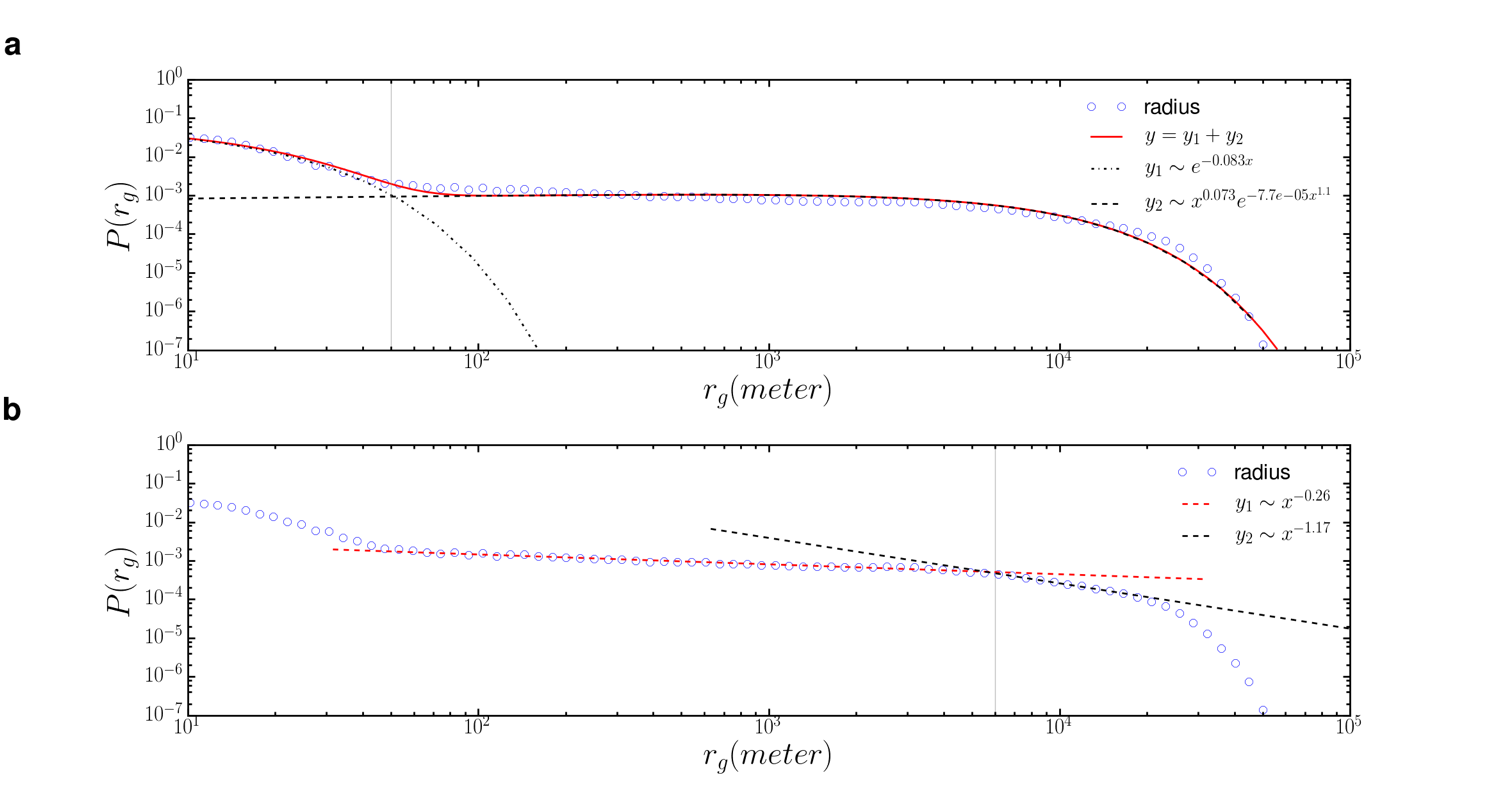
\includegraphics[width=\linewidth]{gyration_chicago}
\caption{Legend (350 words max). Example legend text.}
\label{fig:gyration_chicago}
\end{figure}


\begin{figure}[ht]
\centering
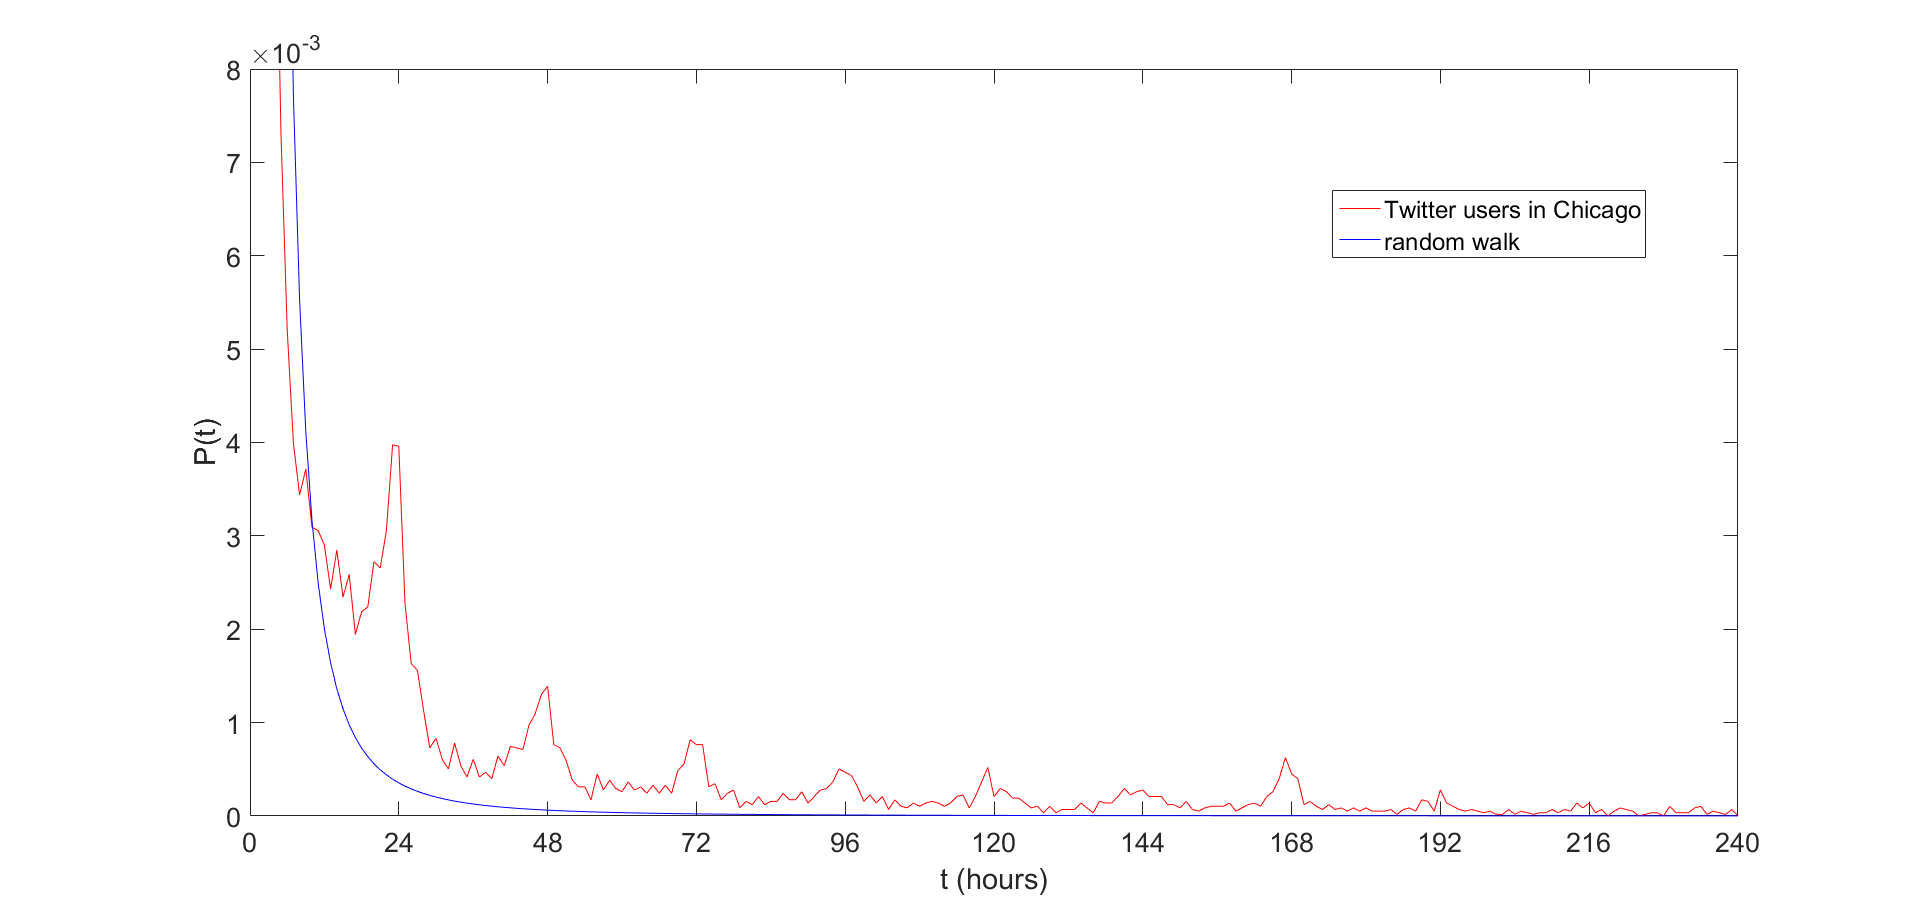
\includegraphics[width=\linewidth]{firsttime}
\caption{First passage time of Twitter user visiting same places}
\label{fig:firsttime}
\end{figure}



\subsection*{Subsection}

Example text under a subsection. Bulleted lists may be used where appropriate, e.g.

\begin{itemize}
\item First item
\item Second item
\end{itemize}

\subsubsection*{Third-level section}
 
Topical subheadings are allowed.

\section*{Discussion}

The Discussion should be succinct and must not contain subheadings.

\section*{Methods}
Contextualizing the semantic meaning of the geo-located tweets

Spatial entropy

Spatial dispersion

Mobility shape

First passage time model



\bibliography{ref}

\section*{Acknowledgements}

Acknowledgements should be brief, and should not include thanks to anonymous referees and editors, or effusive comments. Grant or contribution numbers may be acknowledged.

\section*{Author contributions statement}

Must include all authors, identified by initials, for example:
J.Y. conceived the experiment(s),  J.Y. conducted the experiment(s), J.Y. analysed the results.  All authors reviewed the manuscript. 

\section*{Additional information}
The authors declare no competing financial interests.
\end{document}